\documentclass[12pt]{article}
\usepackage[utf8]{inputenc}
\usepackage[spanish,mexico]{babel}
\usepackage{float}

\usepackage{graphicx}
\graphicspath{{images/}}

\usepackage{vmargin}
\setmarginsrb{3 cm}{2.5 cm}{3 cm}{2.5 cm}{1 cm}{1.5 cm}{1 cm}{1.5 cm}

\begin{document}

\title{Actividad 1: Preparando documentos científicos con LATEX}
\author{Martin Alejandro Paredes Sosa}
\date{Enero 2016}
\maketitle

\section{Péndulo Simple}
Es una idealización de un ``péndulo real" pero aislado utilizando las siguinetes supuestos:
\begin{itemize}
\item El cable o cuerda del péndulo se considera sin masa, no esxtendible y siempre tensa.
\item Es considerada una masa puntua.l %Checar traducción
\item El movimiento es bidimensional(sos direcciones) y sigue al movimiento de un arco.
\item EL movimiento no pierde energia contra la fricción a o resistencia al aire.
\item El campo gravitacional es uniforme.
\item El soporte no se mueve.
\end{itemize}

La ecuación diferencial que representa el movimento del pédulo es la siguiente:
\begin{equation}
\frac{d^2\theta}{dt^2}+\frac{g}{\ell}\sin\theta=0
\end{equation}
donde $g$ es la acerelación debida a la gravedad, $l$ la longitud del péndulo y $\theta$ es el ángulo de desplazamiento.

%\subsection{Derivación de ``Fuerza" de la ecuación 1}
%Usando como referencia a la Figura 1, que muestra las fuerazas que actuan sobre el péndulo. el camino que recorre el péndulo es un arco. El ángulo $\theta$ se mide en radianes lo cual es crucial. La flecha azul representa la fuerza gravitacional, las flechas moradas son la misma fuerza nomas que descompuetas en sus diferentes compentes paralelas y perpendiculares al movimiento en el instante. La direccion de la velociadad instantanea siempre es sobre el eje rojo
%\begin{figure}[H]
%\centering
%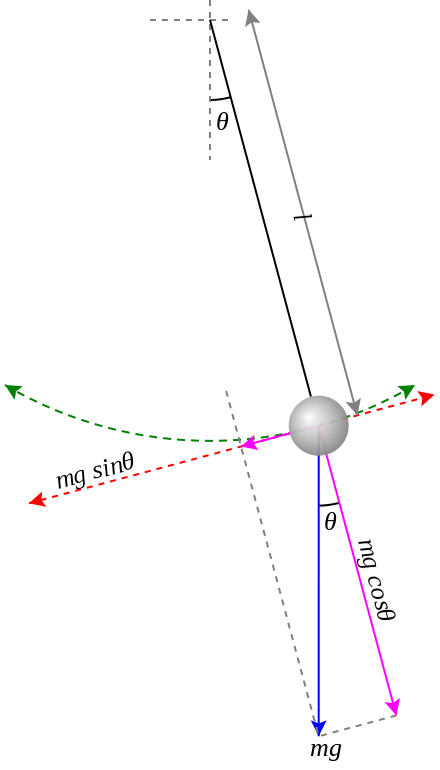
\includegraphics[width=4cm]{pendulo}
%\caption{Diagrama de fuerzas del péndulo simple}
%\end{figure}

\pagebreak
\section{Aproximación con ángulo pequeño}
La ecuación diferencial dada anteriormente no es simple de resolver y no exite solución que pueda ser escrita en terminos de funciones elementales. Pero, si se pone restrición al tamaño de la amplitud de la oscilación nos permite encontrar una solución sencilla. Si se asume que el angulo es mucho menor a un radian, o 
{$$\theta \ll 1$$}
luego se sustituye en (1) usando la aproximación de ángulo pequeño,
{ $$\sin \theta \approx \theta $$}
se obtiene la ecuación de un oscilador armonico,
{ $$\frac{d^2\theta}{dt^2}+\frac{g}{\ell}\theta=0$$}
 El error dado por la aproximación es de orden $\theta^3$.\\
 \\
 Dado la condición inicial $\theta(0)= \theta_0$ y $\frac{d\theta}{dt}(0)=0$, la solucion es:
{ $$\theta(t)= \theta_o \cos \left(\sqrt{\frac{g}{\ell}}t \right) \qquad  \theta_o \ll 1  $$}
El movimeiento es un movimeintos armónico simple donde $\theta_o$ es la semi-amplitud de la oscilación (este es el maximo angulo entre la cuerda del péndulo y la vertical). El periodo del movimiento, el tiempo para completar una oscilación es: 
{$$ T_o=2\pi\sqrt{\frac{\ell}{g}} \qquad  \theta_o \ll 1$$}
a lo que se le conoce como la ley de Christiaan Huygens para el periodo. Note que el ángulo debajo de la aproximación del pequeño ángulo, el periodo es independiente the la amplitud $\theta_o$; esta es la caracteristica de isocronismo que Galileo descubrió.

\subsection{Regla de oro para la longitud del péndulo}
{\large $ T_o=2\pi\sqrt{\frac{\ell}{g}}$} puede ser expresada como {\large$\ell=\frac{g}{\pi^2}\times \frac{T_o^2}{4}$}\\
Si las unidades SI son usadas($\frac{m}{s}$), y asumimos que las mediciones se hacen en la superficie de la tierra, donde {g $\approx$9.81$\frac{m}{s^2}$}, y $g/\pi^2 \approx 1$.

\end{document}